\documentclass[a4paper]{book}
\usepackage{makeidx}
\usepackage{natbib}
\usepackage{graphicx}
\usepackage{multicol}
\usepackage{float}
\usepackage{listings}
\usepackage{color}
\usepackage{ifthen}
\usepackage[table]{xcolor}
\usepackage{textcomp}
\usepackage{alltt}
\usepackage{ifpdf}
\ifpdf
\usepackage[pdftex,
            pagebackref=true,
            colorlinks=true,
            linkcolor=blue,
            unicode
           ]{hyperref}
\else
\usepackage[ps2pdf,
            pagebackref=true,
            colorlinks=true,
            linkcolor=blue,
            unicode
           ]{hyperref}
\usepackage{pspicture}
\fi
\usepackage[utf8]{inputenc}
\usepackage{mathptmx}
\usepackage[scaled=.90]{helvet}
\usepackage{courier}
\usepackage{sectsty}
\usepackage[titles]{tocloft}
\usepackage{doxygen}
\lstset{language=C++,inputencoding=utf8,basicstyle=\footnotesize,breaklines=true,breakatwhitespace=true,tabsize=3,numbers=left }
\makeindex
\setcounter{tocdepth}{3}
\renewcommand{\footrulewidth}{0.4pt}
\renewcommand{\familydefault}{\sfdefault}
\hfuzz=15pt
\setlength{\emergencystretch}{15pt}
\hbadness=750
\tolerance=750
\begin{document}
\hypersetup{pageanchor=false,citecolor=blue}
\begin{titlepage}
\vspace*{7cm}
\begin{center}
{\Large \-Graf\-Onto \\[1ex]\large 0.\-35 }\\
\vspace*{1cm}
{\large \-Generated by Doxygen 1.7.6.1}\\
\vspace*{0.5cm}
{\small Tue Aug 7 2012 23:00:25}\\
\end{center}
\end{titlepage}
\clearemptydoublepage
\pagenumbering{roman}
\tableofcontents
\clearemptydoublepage
\pagenumbering{arabic}
\hypersetup{pageanchor=true,citecolor=blue}
\chapter{\-Class \-Index}
\section{\-Class \-Hierarchy}
\-This inheritance list is sorted roughly, but not completely, alphabetically\-:\begin{DoxyCompactList}
\item \contentsline{section}{mbdev\-\_\-ontology\-:\-:cell}{\pageref{classmbdev__ontology_1_1cell}}{}
\item \contentsline{section}{mbdev\-:\-:console\-\_\-application}{\pageref{classmbdev_1_1console__application}}{}
\begin{DoxyCompactList}
\item \contentsline{section}{grafonto}{\pageref{classgrafonto}}{}
\end{DoxyCompactList}
\item \contentsline{section}{\-Main\-Window}{\pageref{class_main_window}}{}
\item \contentsline{section}{mbdev\-\_\-ontology\-:\-:node}{\pageref{classmbdev__ontology_1_1node}}{}
\begin{DoxyCompactList}
\item \contentsline{section}{mbdev\-\_\-ontology\-:\-:category}{\pageref{classmbdev__ontology_1_1category}}{}
\item \contentsline{section}{mbdev\-\_\-ontology\-:\-:element}{\pageref{classmbdev__ontology_1_1element}}{}
\end{DoxyCompactList}
\item \contentsline{section}{mbdev\-\_\-ontology\-:\-:ontology}{\pageref{classmbdev__ontology_1_1ontology}}{}
\item \contentsline{section}{mbdev\-\_\-ontology\-:\-:statement}{\pageref{classmbdev__ontology_1_1statement}}{}
\item \contentsline{section}{mbdev\-:\-:string}{\pageref{classmbdev_1_1string}}{}
\item \contentsline{section}{vector}{\pageref{classstd_1_1vector}}{}
\begin{DoxyCompactList}
\item \contentsline{section}{mbdev\-:\-:vector$<$ \-T $>$}{\pageref{classmbdev_1_1vector}}{}
\item \contentsline{section}{mbdev\-:\-:vector$<$ string $>$}{\pageref{classmbdev_1_1vector}}{}
\begin{DoxyCompactList}
\item \contentsline{section}{mbdev\-:\-:string\-\_\-vector}{\pageref{classmbdev_1_1string__vector}}{}
\end{DoxyCompactList}
\item \contentsline{section}{mbdev\-:\-:vector$<$ \-T $\ast$ $>$}{\pageref{classmbdev_1_1vector}}{}
\begin{DoxyCompactList}
\item \contentsline{section}{mbdev\-:\-:ptr\-\_\-vector$<$ \-T $>$}{\pageref{classmbdev_1_1ptr__vector}}{}
\end{DoxyCompactList}
\end{DoxyCompactList}
\end{DoxyCompactList}

\chapter{\-Class \-Index}
\section{\-Class \-List}
\-Here are the classes, structs, unions and interfaces with brief descriptions\-:\begin{DoxyCompactList}
\item\contentsline{section}{\hyperlink{class_category}{\-Category} \\*\-Defines a property than an \hyperlink{class_element}{\-Element} can have }{\pageref{class_category}}{}
\item\contentsline{section}{\hyperlink{class_element}{\-Element} \\*\hyperlink{class_element}{\-Element} stores a value of a specific \hyperlink{class_category}{\-Category}. \-Value may affect other values of the \-Cell containing it, as well as \-Cells connected to the above mentioned cell }{\pageref{class_element}}{}
\item\contentsline{section}{\hyperlink{class_main_window}{\-Main\-Window} }{\pageref{class_main_window}}{}
\item\contentsline{section}{\hyperlink{class_node}{\-Node} \\*\-Contains common behaviour of \hyperlink{class_element}{\-Element} and \-Relation }{\pageref{class_node}}{}
\item\contentsline{section}{\hyperlink{class_ontology}{\-Ontology} \\*\-A network of possibly connected concepts. \-Concepts are organized into \-Elements, and these are organized into \-Categories. \-Each \hyperlink{class_element}{\-Element} belongs to exactly one \hyperlink{class_category}{\-Category}. \-Elements are then joined together into groups called \-Cells. \-A \-Cell contains at most one element of every category defined in the ontology }{\pageref{class_ontology}}{}
\item\contentsline{section}{\hyperlink{class_strings}{\-Strings} \\*\-Utility class used to handle strings and vectors of strings }{\pageref{class_strings}}{}
\end{DoxyCompactList}

\chapter{\-Class \-Documentation}
\hypertarget{classmbdev__ontology_1_1category}{\section{mbdev\-\_\-ontology\-:\-:category \-Class \-Reference}
\label{classmbdev__ontology_1_1category}\index{mbdev\-\_\-ontology\-::category@{mbdev\-\_\-ontology\-::category}}
}


\-Defines a property than an \-Element can have.  




{\ttfamily \#include $<$category.\-h$>$}

\-Inheritance diagram for mbdev\-\_\-ontology\-:\-:category\-:\begin{figure}[H]
\begin{center}
\leavevmode
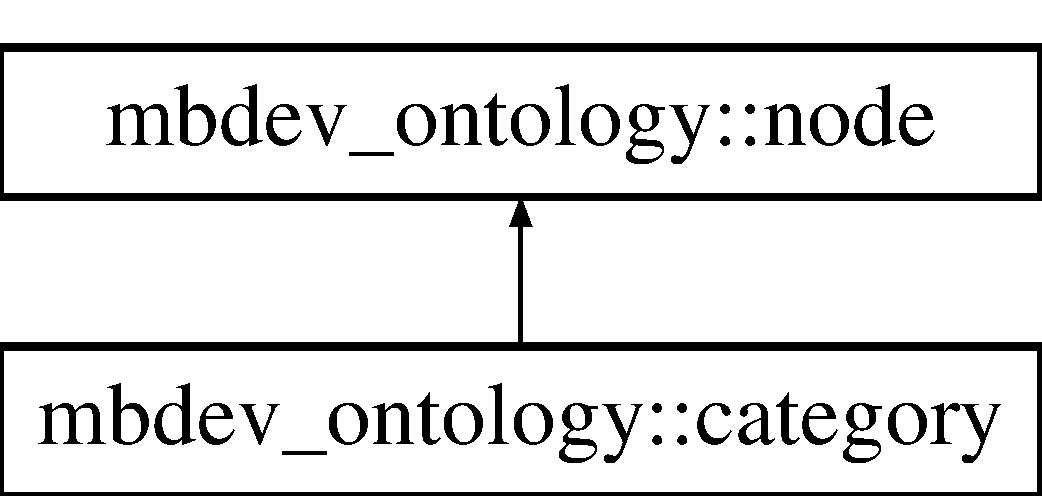
\includegraphics[height=2.000000cm]{classmbdev__ontology_1_1category}
\end{center}
\end{figure}
\subsection*{\-Public \-Member \-Functions}
\begin{DoxyCompactItemize}
\item 
\hypertarget{classmbdev__ontology_1_1category_a742d5330d357001324311141fa90fd49}{{\bfseries category} (\hyperlink{classmbdev_1_1string}{string} \&\hyperlink{classmbdev__ontology_1_1node_a0f69893fcec007d0766997400830a204}{name})}\label{classmbdev__ontology_1_1category_a742d5330d357001324311141fa90fd49}

\item 
\hypertarget{classmbdev__ontology_1_1category_aab41d47f57bb6e732febc0d9cc80eb18}{{\bfseries category} (\hyperlink{classmbdev_1_1string}{string} \&\hyperlink{classmbdev__ontology_1_1node_a0f69893fcec007d0766997400830a204}{name}, \hyperlink{classmbdev_1_1string}{string} \&\hyperlink{classmbdev__ontology_1_1node_a8af5c00f684a8c06ceeddd0a2b1ff97c}{friendly\-Name})}\label{classmbdev__ontology_1_1category_aab41d47f57bb6e732febc0d9cc80eb18}

\end{DoxyCompactItemize}


\subsection{\-Detailed \-Description}
\-Defines a property than an \-Element can have. 

\-The documentation for this class was generated from the following files\-:\begin{DoxyCompactItemize}
\item 
/media/projects/cpp/\-Graf\-Onto/src/ontology/category.\-h\item 
/media/projects/cpp/\-Graf\-Onto/src/ontology/category.\-cpp\end{DoxyCompactItemize}

\hypertarget{classmbdev__ontology_1_1cell}{\section{mbdev\-\_\-ontology\-:\-:cell \-Class \-Reference}
\label{classmbdev__ontology_1_1cell}\index{mbdev\-\_\-ontology\-::cell@{mbdev\-\_\-ontology\-::cell}}
}


\-Used to store a set of elements, each of which belonging to a different category. \-Uses a map\-: a structure that contains at most one value for each category defined in the ontology.  




{\ttfamily \#include $<$cell.\-h$>$}

\subsection*{\-Public \-Member \-Functions}
\begin{DoxyCompactItemize}
\item 
\hypertarget{classmbdev__ontology_1_1cell_ab940fc0fd635d5d6924bf7a8ba7acb3d}{{\bfseries cell} (const \hyperlink{classmbdev_1_1string__vector}{string\-\_\-vector} \&vec, \hyperlink{classmbdev__ontology_1_1ontology}{ontology} \&onto)}\label{classmbdev__ontology_1_1cell_ab940fc0fd635d5d6924bf7a8ba7acb3d}

\item 
\hypertarget{classmbdev__ontology_1_1cell_ae19060aca87c166b4e4beeda191f79a9}{void {\bfseries insert} (\hyperlink{classmbdev__ontology_1_1element}{element} $\ast$e)}\label{classmbdev__ontology_1_1cell_ae19060aca87c166b4e4beeda191f79a9}

\item 
\hypertarget{classmbdev__ontology_1_1cell_aa9d59dd81d6576eaeda7710dbe1287d3}{void {\bfseries insert} (\hyperlink{classmbdev__ontology_1_1category}{category} $\ast$c, \hyperlink{classmbdev__ontology_1_1element}{element} $\ast$e)}\label{classmbdev__ontology_1_1cell_aa9d59dd81d6576eaeda7710dbe1287d3}

\end{DoxyCompactItemize}
\subsection*{\-Friends}
\begin{DoxyCompactItemize}
\item 
\hypertarget{classmbdev__ontology_1_1cell_a89fd6ed708bc15412d8b747802499dc9}{std\-::ostream \& {\bfseries operator$<$$<$} (std\-::ostream \&os, const \hyperlink{classmbdev__ontology_1_1cell}{cell} \&c)}\label{classmbdev__ontology_1_1cell_a89fd6ed708bc15412d8b747802499dc9}

\end{DoxyCompactItemize}


\subsection{\-Detailed \-Description}
\-Used to store a set of elements, each of which belonging to a different category. \-Uses a map\-: a structure that contains at most one value for each category defined in the ontology. 

\-The documentation for this class was generated from the following files\-:\begin{DoxyCompactItemize}
\item 
/media/projects/cpp/\-Graf\-Onto/src/ontology/cell.\-h\item 
/media/projects/cpp/\-Graf\-Onto/src/ontology/cell.\-cpp\end{DoxyCompactItemize}

\hypertarget{classmbdev_1_1console__application}{\section{mbdev\-:\-:console\-\_\-application \-Class \-Reference}
\label{classmbdev_1_1console__application}\index{mbdev\-::console\-\_\-application@{mbdev\-::console\-\_\-application}}
}


\-Meant to be sub-\/classed with a real console application.  




{\ttfamily \#include $<$console\-\_\-application.\-h$>$}

\-Inheritance diagram for mbdev\-:\-:console\-\_\-application\-:\begin{figure}[H]
\begin{center}
\leavevmode
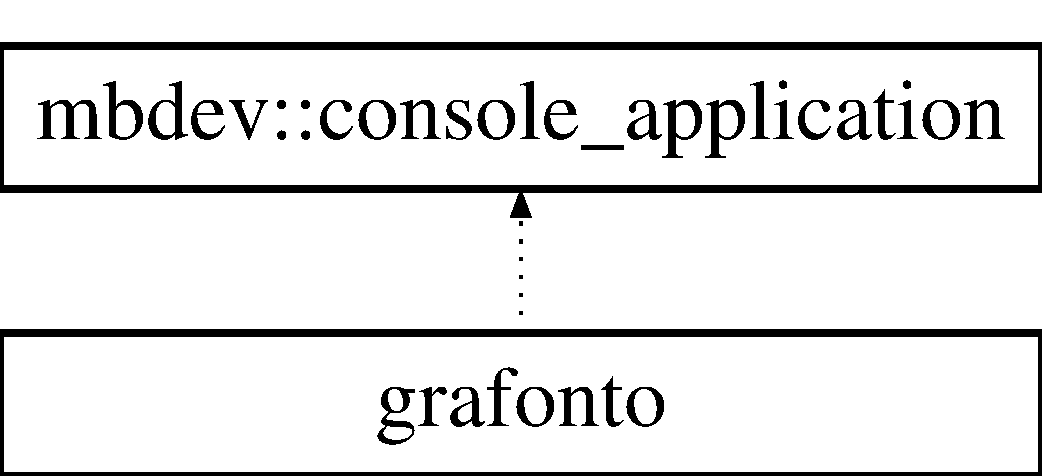
\includegraphics[height=2.000000cm]{classmbdev_1_1console__application}
\end{center}
\end{figure}
\subsection*{\-Public \-Member \-Functions}
\begin{DoxyCompactItemize}
\item 
\hypertarget{classmbdev_1_1console__application_a3ec9a999cbcb3be3f27ace507b18edb2}{{\bfseries console\-\_\-application} (int argc, char $\ast$argv\mbox{[}$\,$\mbox{]}, std\-::ostream \&output\-Stream=std\-::cout)}\label{classmbdev_1_1console__application_a3ec9a999cbcb3be3f27ace507b18edb2}

\item 
\hypertarget{classmbdev_1_1console__application_ad157a0ef8d992092b8d9d14e7f621073}{\hyperlink{classmbdev_1_1string}{string} {\bfseries get\-User\-Symbol} () const }\label{classmbdev_1_1console__application_ad157a0ef8d992092b8d9d14e7f621073}

\item 
\hypertarget{classmbdev_1_1console__application_a311506abcf542bc78385f447171b3b7d}{size\-\_\-t {\bfseries get\-Command\-History\-Size} () const }\label{classmbdev_1_1console__application_a311506abcf542bc78385f447171b3b7d}

\item 
\hypertarget{classmbdev_1_1console__application_af0c2e1dc86119c3da094dd00a0c6bdb2}{\hyperlink{classmbdev_1_1string}{string} {\bfseries get\-Command\-History\-Entry} (const size\-\_\-t index) const }\label{classmbdev_1_1console__application_af0c2e1dc86119c3da094dd00a0c6bdb2}

\item 
\hypertarget{classmbdev_1_1console__application_a58242f26b9b2b32faa2525bea0f6eecd}{bool {\bfseries is\-Allowed} (char ch)}\label{classmbdev_1_1console__application_a58242f26b9b2b32faa2525bea0f6eecd}

\item 
\hypertarget{classmbdev_1_1console__application_aaf462b9a5c8764896c8c2bf2f12271e1}{\hyperlink{classmbdev_1_1string}{string} {\bfseries extern\-Execute} (const \hyperlink{classmbdev_1_1string}{string} \&command)}\label{classmbdev_1_1console__application_aaf462b9a5c8764896c8c2bf2f12271e1}

\item 
\hypertarget{classmbdev_1_1console__application_a4da56afaaaf53820dde5551ae34bc8da}{virtual int {\bfseries exec} ()}\label{classmbdev_1_1console__application_a4da56afaaaf53820dde5551ae34bc8da}

\item 
\hypertarget{classmbdev_1_1console__application_aaba2a906eb64593cc43ceec6ad96e830}{int {\bfseries simulate\-Exec} (const \hyperlink{classmbdev_1_1string}{string} \&input)}\label{classmbdev_1_1console__application_aaba2a906eb64593cc43ceec6ad96e830}

\end{DoxyCompactItemize}
\subsection*{\-Protected \-Member \-Functions}
\begin{DoxyCompactItemize}
\item 
\hypertarget{classmbdev_1_1console__application_a8dc3fef0a026cb33b71b08ae3a02c9fd}{void {\bfseries handle\-Tab} (\hyperlink{classmbdev_1_1string}{string} \&text)}\label{classmbdev_1_1console__application_a8dc3fef0a026cb33b71b08ae3a02c9fd}

\item 
\hypertarget{classmbdev_1_1console__application_ac6bd452145f850e141c3ca64f401c04c}{virtual \hyperlink{classmbdev_1_1string}{string} {\bfseries execute} (const \hyperlink{classmbdev_1_1string}{string} \&command)}\label{classmbdev_1_1console__application_ac6bd452145f850e141c3ca64f401c04c}

\item 
\hypertarget{classmbdev_1_1console__application_a518e890cc969a5986d171dea2e800115}{virtual \hyperlink{classmbdev_1_1string}{string} {\bfseries get\-Clue} (const \hyperlink{classmbdev_1_1string}{string} \&current)}\label{classmbdev_1_1console__application_a518e890cc969a5986d171dea2e800115}

\item 
\hyperlink{classmbdev_1_1string}{string} \hyperlink{classmbdev_1_1console__application_a7d13549416b40695a144fd1f3eb999bc}{get\-Command} ()
\begin{DoxyCompactList}\small\item\em \-Blocks the console and waits for user input. \end{DoxyCompactList}\item 
\hypertarget{classmbdev_1_1console__application_a045e4f99a41e470c5e2f85cfce5d65a8}{\hyperlink{classmbdev_1_1string}{string} {\bfseries get\-Simulated\-Command} (const \hyperlink{classmbdev_1_1string}{string} \&simulated)}\label{classmbdev_1_1console__application_a045e4f99a41e470c5e2f85cfce5d65a8}

\end{DoxyCompactItemize}
\subsection*{\-Protected \-Attributes}
\begin{DoxyCompactItemize}
\item 
\hypertarget{classmbdev_1_1console__application_ae43acd48296ae5e210c63f4bcf79a348}{bool {\bfseries debug\-Mode}}\label{classmbdev_1_1console__application_ae43acd48296ae5e210c63f4bcf79a348}

\item 
\hypertarget{classmbdev_1_1console__application_a9fd2e56ecae607129169af845dc85174}{int {\bfseries argc}}\label{classmbdev_1_1console__application_a9fd2e56ecae607129169af845dc85174}

\item 
\hypertarget{classmbdev_1_1console__application_a92abff8076aa6963cb3f513510cd8257}{char $\ast$$\ast$ {\bfseries argv}}\label{classmbdev_1_1console__application_a92abff8076aa6963cb3f513510cd8257}

\item 
\hypertarget{classmbdev_1_1console__application_a9fea8a17d4c76f544deec3817a031587}{\hyperlink{classmbdev_1_1string__vector}{string\-\_\-vector} {\bfseries args}}\label{classmbdev_1_1console__application_a9fea8a17d4c76f544deec3817a031587}

\end{DoxyCompactItemize}


\subsection{\-Detailed \-Description}
\-Meant to be sub-\/classed with a real console application. 

\subsection{\-Member \-Function \-Documentation}
\hypertarget{classmbdev_1_1console__application_a7d13549416b40695a144fd1f3eb999bc}{\index{mbdev\-::console\-\_\-application@{mbdev\-::console\-\_\-application}!get\-Command@{get\-Command}}
\index{get\-Command@{get\-Command}!mbdev::console_application@{mbdev\-::console\-\_\-application}}
\subsubsection[{get\-Command}]{\setlength{\rightskip}{0pt plus 5cm}{\bf string} {\bf mbdev\-::console\-\_\-application\-::get\-Command} (
\begin{DoxyParamCaption}
{}
\end{DoxyParamCaption}
)\hspace{0.3cm}{\ttfamily  \mbox{[}protected\mbox{]}}}}\label{classmbdev_1_1console__application_a7d13549416b40695a144fd1f3eb999bc}


\-Blocks the console and waits for user input. 

\begin{DoxyReturn}{\-Returns}
user command, after pressing \-Enter 
\end{DoxyReturn}


\-The documentation for this class was generated from the following files\-:\begin{DoxyCompactItemize}
\item 
/media/projects/cpp/\-Graf\-Onto/src/mbdev/console\-\_\-application.\-h\item 
/media/projects/cpp/\-Graf\-Onto/src/mbdev/console\-\_\-application.\-cpp\end{DoxyCompactItemize}

\hypertarget{classmbdev__ontology_1_1element}{\section{mbdev\-\_\-ontology\-:\-:element \-Class \-Reference}
\label{classmbdev__ontology_1_1element}\index{mbdev\-\_\-ontology\-::element@{mbdev\-\_\-ontology\-::element}}
}


\-Element stores a value of a specific \-Category. \-Value may affect other values of the \-Cell containing it, as well as \-Cells connected to the above mentioned cell.  




{\ttfamily \#include $<$element.\-h$>$}

\-Inheritance diagram for mbdev\-\_\-ontology\-:\-:element\-:\begin{figure}[H]
\begin{center}
\leavevmode
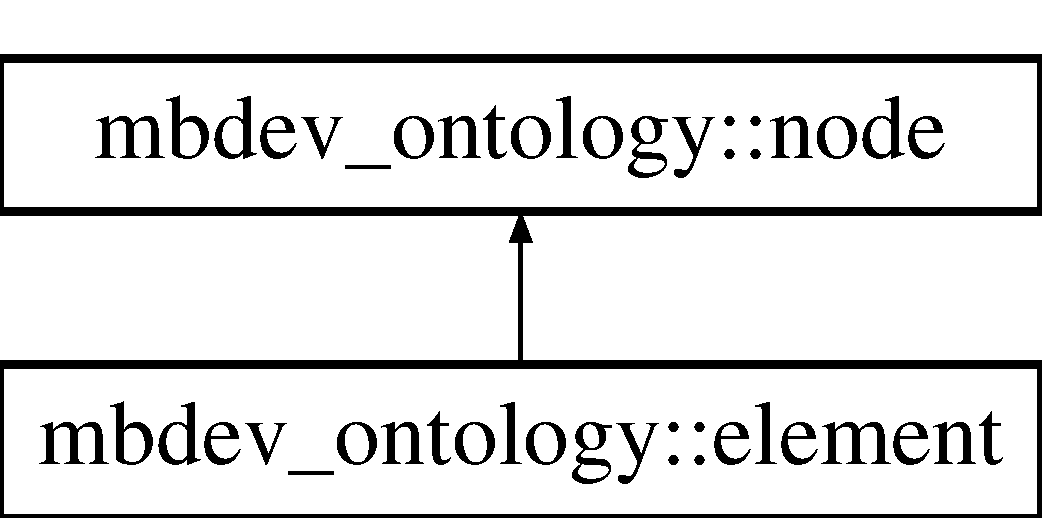
\includegraphics[height=2.000000cm]{classmbdev__ontology_1_1element}
\end{center}
\end{figure}
\subsection*{\-Public \-Member \-Functions}
\begin{DoxyCompactItemize}
\item 
\hypertarget{classmbdev__ontology_1_1element_a1314f373fcfc0e4f8621e7272c7f96f1}{{\bfseries element} (\hyperlink{classmbdev_1_1string}{string} \&\hyperlink{classmbdev__ontology_1_1node_a0f69893fcec007d0766997400830a204}{name}, \hyperlink{classmbdev__ontology_1_1category}{category} $\ast$\hyperlink{classmbdev__ontology_1_1element_a90da561e20a92103b33e879e78032e0a}{cat}, bool \hyperlink{classmbdev__ontology_1_1element_a2dd58a46bab19cdf0c243bcd84c23fdb}{transitive}=false)}\label{classmbdev__ontology_1_1element_a1314f373fcfc0e4f8621e7272c7f96f1}

\item 
\hypertarget{classmbdev__ontology_1_1element_ad50e1b6aa536a204bd6a47ca0cbc5754}{{\bfseries element} (\hyperlink{classmbdev_1_1string}{string} \&\hyperlink{classmbdev__ontology_1_1node_a0f69893fcec007d0766997400830a204}{name}, \hyperlink{classmbdev_1_1string}{string} \&\hyperlink{classmbdev__ontology_1_1node_a8af5c00f684a8c06ceeddd0a2b1ff97c}{friendly\-Name}, \hyperlink{classmbdev__ontology_1_1category}{category} $\ast$\hyperlink{classmbdev__ontology_1_1element_a90da561e20a92103b33e879e78032e0a}{cat}, bool \hyperlink{classmbdev__ontology_1_1element_a2dd58a46bab19cdf0c243bcd84c23fdb}{transitive}=false)}\label{classmbdev__ontology_1_1element_ad50e1b6aa536a204bd6a47ca0cbc5754}

\item 
\hypertarget{classmbdev__ontology_1_1element_ad61d2fbc29f304a342a24080f2950769}{\hyperlink{classmbdev__ontology_1_1category}{category} {\bfseries get\-Category} () const }\label{classmbdev__ontology_1_1element_ad61d2fbc29f304a342a24080f2950769}

\item 
\hypertarget{classmbdev__ontology_1_1element_a3edbfba48add185625a883daab537a4a}{\hyperlink{classmbdev__ontology_1_1category}{category} $\ast$ {\bfseries get\-Category\-Ptr} ()}\label{classmbdev__ontology_1_1element_a3edbfba48add185625a883daab537a4a}

\item 
\hypertarget{classmbdev__ontology_1_1element_a661134a04667b21be53139bf5a73deef}{bool {\bfseries is\-Transitive} () const }\label{classmbdev__ontology_1_1element_a661134a04667b21be53139bf5a73deef}

\item 
\hypertarget{classmbdev__ontology_1_1element_ae4ae80555e858025b5bb8eeff2d44bac}{void {\bfseries set\-Transitive} (bool is\-Transitive)}\label{classmbdev__ontology_1_1element_ae4ae80555e858025b5bb8eeff2d44bac}

\end{DoxyCompactItemize}
\subsection*{\-Protected \-Attributes}
\begin{DoxyCompactItemize}
\item 
\hypertarget{classmbdev__ontology_1_1element_a90da561e20a92103b33e879e78032e0a}{\hyperlink{classmbdev__ontology_1_1category}{category} $\ast$ \hyperlink{classmbdev__ontology_1_1element_a90da561e20a92103b33e879e78032e0a}{cat}}\label{classmbdev__ontology_1_1element_a90da561e20a92103b33e879e78032e0a}

\begin{DoxyCompactList}\small\item\em determines what kind of \-Element it is i.\-e. 'thing', 'situation', etc. \end{DoxyCompactList}\item 
bool \hyperlink{classmbdev__ontology_1_1element_a2dd58a46bab19cdf0c243bcd84c23fdb}{transitive}
\begin{DoxyCompactList}\small\item\em determines if this element is transitive, i.\-e. if\-: 1) three \-Cells are connected like a-\/$>$b-\/$>$c 2) both \-Cell a and \-Cell b have this element in them then the ontology interprets this as if there was a connection between a and c (a-\/$>$c) \end{DoxyCompactList}\end{DoxyCompactItemize}
\subsection*{\-Friends}
\begin{DoxyCompactItemize}
\item 
\hypertarget{classmbdev__ontology_1_1element_aec34156b3910eda665d18dcfe5e2cfe5}{std\-::ostream \& {\bfseries operator$<$$<$} (std\-::ostream \&os, const \hyperlink{classmbdev__ontology_1_1element}{element} \&e)}\label{classmbdev__ontology_1_1element_aec34156b3910eda665d18dcfe5e2cfe5}

\end{DoxyCompactItemize}


\subsection{\-Detailed \-Description}
\-Element stores a value of a specific \-Category. \-Value may affect other values of the \-Cell containing it, as well as \-Cells connected to the above mentioned cell. 

\subsection{\-Member \-Data \-Documentation}
\hypertarget{classmbdev__ontology_1_1element_a2dd58a46bab19cdf0c243bcd84c23fdb}{\index{mbdev\-\_\-ontology\-::element@{mbdev\-\_\-ontology\-::element}!transitive@{transitive}}
\index{transitive@{transitive}!mbdev_ontology::element@{mbdev\-\_\-ontology\-::element}}
\subsubsection[{transitive}]{\setlength{\rightskip}{0pt plus 5cm}bool {\bf mbdev\-\_\-ontology\-::element\-::transitive}\hspace{0.3cm}{\ttfamily  \mbox{[}protected\mbox{]}}}}\label{classmbdev__ontology_1_1element_a2dd58a46bab19cdf0c243bcd84c23fdb}


determines if this element is transitive, i.\-e. if\-: 1) three \-Cells are connected like a-\/$>$b-\/$>$c 2) both \-Cell a and \-Cell b have this element in them then the ontology interprets this as if there was a connection between a and c (a-\/$>$c) 

example ontology\-: \char`\"{}add category obj\char`\"{} \char`\"{}add category relation\char`\"{} \char`\"{}add obj a\char`\"{} \char`\"{}add obj b\char`\"{} \char`\"{}add obj c\char`\"{} \char`\"{}add relation is\char`\"{} \char`\"{}set is transitive\char`\"{} \char`\"{}a is\-: b\char`\"{} \char`\"{}b is\-: c\char`\"{} query\-: \char`\"{}find all that is c\char`\"{} program responds\-: \char`\"{}\mbox{[}obj\-:a, obj\-:b\mbox{]}\char`\"{} 

\-The documentation for this class was generated from the following files\-:\begin{DoxyCompactItemize}
\item 
/media/projects/cpp/\-Graf\-Onto/src/ontology/element.\-h\item 
/media/projects/cpp/\-Graf\-Onto/src/ontology/element.\-cpp\end{DoxyCompactItemize}

\hypertarget{classgrafonto}{\section{grafonto \-Class \-Reference}
\label{classgrafonto}\index{grafonto@{grafonto}}
}
\-Inheritance diagram for grafonto\-:\begin{figure}[H]
\begin{center}
\leavevmode
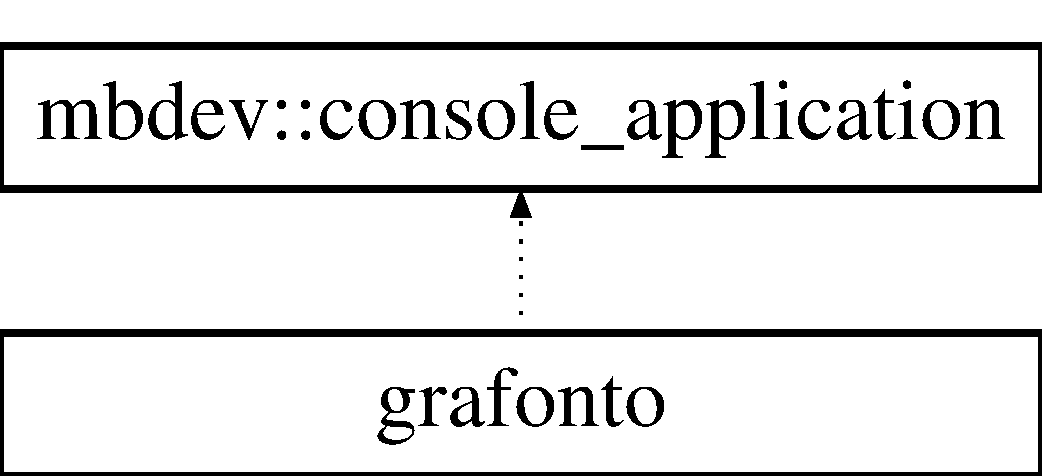
\includegraphics[height=2.000000cm]{classgrafonto}
\end{center}
\end{figure}
\subsection*{\-Public \-Member \-Functions}
\begin{DoxyCompactItemize}
\item 
\hypertarget{classgrafonto_ac24e7e64810ed10cf36656bd7e8e9b12}{{\bfseries grafonto} (int argc, char $\ast$argv\mbox{[}$\,$\mbox{]})}\label{classgrafonto_ac24e7e64810ed10cf36656bd7e8e9b12}

\item 
\hypertarget{classgrafonto_a3f2cce1c012b25e0c66ec2bbdbc3f786}{virtual int {\bfseries exec} ()}\label{classgrafonto_a3f2cce1c012b25e0c66ec2bbdbc3f786}

\item 
\hypertarget{classgrafonto_adfef5ece0152a2c3715eacab7a7673af}{int {\bfseries text\-\_\-mode} ()}\label{classgrafonto_adfef5ece0152a2c3715eacab7a7673af}

\item 
\hypertarget{classgrafonto_ac2ab48fb386a5814d3270e3c70877a16}{int {\bfseries gui\-\_\-mode} ()}\label{classgrafonto_ac2ab48fb386a5814d3270e3c70877a16}

\end{DoxyCompactItemize}
\subsection*{\-Protected \-Member \-Functions}
\begin{DoxyCompactItemize}
\item 
\hypertarget{classgrafonto_a638219f0ede60ecdd4563759e8610af2}{\hyperlink{classmbdev_1_1string}{string} {\bfseries execute\-Add} (\hyperlink{classmbdev_1_1string__vector}{string\-\_\-vector} \&arguments)}\label{classgrafonto_a638219f0ede60ecdd4563759e8610af2}

\item 
\hypertarget{classgrafonto_ad23ffa340d8adfd8d7d124cfbc2acd5a}{\hyperlink{classmbdev_1_1string}{string} {\bfseries execute\-Set} (\hyperlink{classmbdev_1_1string__vector}{string\-\_\-vector} \&arguments)}\label{classgrafonto_ad23ffa340d8adfd8d7d124cfbc2acd5a}

\item 
\hypertarget{classgrafonto_a70dd25b1813816cf86ce1a648ea73bf6}{\hyperlink{classmbdev_1_1string}{string} {\bfseries execute\-Delete} (\hyperlink{classmbdev_1_1string__vector}{string\-\_\-vector} \&arguments)}\label{classgrafonto_a70dd25b1813816cf86ce1a648ea73bf6}

\item 
\hypertarget{classgrafonto_a830c6f5519f944c6ef2eeff41b614ec1}{\hyperlink{classmbdev_1_1string}{string} {\bfseries execute\-Find} (\hyperlink{classmbdev_1_1string__vector}{string\-\_\-vector} \&arguments)}\label{classgrafonto_a830c6f5519f944c6ef2eeff41b614ec1}

\item 
\hypertarget{classgrafonto_a3f68ed8a56cb970d74213b46f9c79446}{\hyperlink{classmbdev_1_1string}{string} {\bfseries execute\-Load} (\hyperlink{classmbdev_1_1string__vector}{string\-\_\-vector} \&arguments)}\label{classgrafonto_a3f68ed8a56cb970d74213b46f9c79446}

\item 
\hypertarget{classgrafonto_a160a47eeb7221a3b7cebb677f097918c}{\hyperlink{classmbdev_1_1string}{string} {\bfseries execute\-Save} (\hyperlink{classmbdev_1_1string__vector}{string\-\_\-vector} \&arguments)}\label{classgrafonto_a160a47eeb7221a3b7cebb677f097918c}

\item 
\hypertarget{classgrafonto_a7ff5a6e85553906cef2126f3d5ffa8e2}{\hyperlink{classmbdev_1_1string}{string} {\bfseries execute\-Statement} (\hyperlink{classmbdev_1_1string__vector}{string\-\_\-vector} \&arguments)}\label{classgrafonto_a7ff5a6e85553906cef2126f3d5ffa8e2}

\item 
virtual \hyperlink{classmbdev_1_1string}{string} \hyperlink{classgrafonto_ab0d713e50d84c78a2dc6c7d190beaeae}{execute} (const \hyperlink{classmbdev_1_1string}{string} \&command)
\begin{DoxyCompactList}\small\item\em \-Executes a command on the ontology. \end{DoxyCompactList}\item 
\hypertarget{classgrafonto_a52ec25f316e0d0c2d49bfaa52b815a96}{virtual \hyperlink{classmbdev_1_1string}{string} {\bfseries get\-Clue} (const \hyperlink{classmbdev_1_1string}{string} \&current)}\label{classgrafonto_a52ec25f316e0d0c2d49bfaa52b815a96}

\end{DoxyCompactItemize}


\subsection{\-Member \-Function \-Documentation}
\hypertarget{classgrafonto_ab0d713e50d84c78a2dc6c7d190beaeae}{\index{grafonto@{grafonto}!execute@{execute}}
\index{execute@{execute}!grafonto@{grafonto}}
\subsubsection[{execute}]{\setlength{\rightskip}{0pt plus 5cm}{\bf string} {\bf grafonto\-::execute} (
\begin{DoxyParamCaption}
\item[{const {\bf string} \&}]{command}
\end{DoxyParamCaption}
)\hspace{0.3cm}{\ttfamily  \mbox{[}protected, virtual\mbox{]}}}}\label{classgrafonto_ab0d713e50d84c78a2dc6c7d190beaeae}


\-Executes a command on the ontology. 


\begin{DoxyParams}{\-Parameters}
{\em command} & natural language command given as a parameter, which is parsed, analyzed and executed; operation is aborted in case of any error in command; example commands\-: to add a category 'thing'\-: 
\begin{DoxyCode}
 add category thing 
\end{DoxyCode}
 to delete a category 'thing'\-: 
\begin{DoxyCode}
 delete category thing 
\end{DoxyCode}
 to add an element of category 'thing', named 'car' 
\begin{DoxyCode}
 add thing car 
\end{DoxyCode}
 to add a relation 'is' (assuming category named 'relation' exists)\-: 
\begin{DoxyCode}
 add relation is 
\end{DoxyCode}
 to make relation 'is' transitive\-: 
\begin{DoxyCode}
 set is transitive 
\end{DoxyCode}
 to make relation 'is' not transitive (which is a default for every element)\-: 
\begin{DoxyCode}
 set is not transitive 
\end{DoxyCode}
 to add a connection (assuming things 'car' and 'vehicle' exist, and relation 'is' exists)\-: 
\begin{DoxyCode}
 car is: vehicle 
\end{DoxyCode}
 to find every element that 'is animal'\-: 
\begin{DoxyCode}
 find all that is animal 
\end{DoxyCode}
 to find every 'thing' that 'has wings'\-: 
\begin{DoxyCode}
 find thing that has wings 
\end{DoxyCode}
 \\
\hline
\end{DoxyParams}
\begin{DoxyReturn}{\-Returns}
result of the command, which non-\/empty only in case of queries. queries are done using 'find' keyword, for example, given an ontology\-: 
\begin{DoxyCode}
 add category (obj, relation)
      add obj (a, b, c)
      add relation is
      set is transitive
      a is: b
      b is: c
\end{DoxyCode}
 by executing the command 
\begin{DoxyCode}
 find all that is c 
\end{DoxyCode}
 program returns 
\begin{DoxyCode}
 a, b 
\end{DoxyCode}
 
\end{DoxyReturn}


\-Reimplemented from \hyperlink{classmbdev_1_1console__application}{mbdev\-::console\-\_\-application}.



\-The documentation for this class was generated from the following files\-:\begin{DoxyCompactItemize}
\item 
/media/projects/cpp/\-Graf\-Onto/src/grafonto.\-h\item 
/media/projects/cpp/\-Graf\-Onto/src/grafonto.\-cpp\end{DoxyCompactItemize}

\hypertarget{class_main_window}{\section{\-Main\-Window \-Class \-Reference}
\label{class_main_window}\index{\-Main\-Window@{\-Main\-Window}}
}


\-Main window consists of two parts, command line with log on the left, and ontology visualisation area on the right hand side.  




{\ttfamily \#include $<$mainwindow.\-h$>$}

\subsection*{\-Public \-Member \-Functions}
\begin{DoxyCompactItemize}
\item 
\hyperlink{class_main_window_a76ffb9279211c23d2a54f2bced90da85}{\-Main\-Window} (\hyperlink{classmbdev__ontology_1_1ontology}{ontology} \&onto, \-Q\-Application \&app, \-Q\-Widget $\ast$parent=0)
\begin{DoxyCompactList}\small\item\em \-Constructs the main window of \-Graf\-Onto. \end{DoxyCompactList}\end{DoxyCompactItemize}


\subsection{\-Detailed \-Description}
\-Main window consists of two parts, command line with log on the left, and ontology visualisation area on the right hand side. 

\subsection{\-Constructor \& \-Destructor \-Documentation}
\hypertarget{class_main_window_a76ffb9279211c23d2a54f2bced90da85}{\index{\-Main\-Window@{\-Main\-Window}!\-Main\-Window@{\-Main\-Window}}
\index{\-Main\-Window@{\-Main\-Window}!MainWindow@{\-Main\-Window}}
\subsubsection[{\-Main\-Window}]{\setlength{\rightskip}{0pt plus 5cm}{\bf \-Main\-Window\-::\-Main\-Window} (
\begin{DoxyParamCaption}
\item[{{\bf ontology} \&}]{onto, }
\item[{\-Q\-Application \&}]{app, }
\item[{\-Q\-Widget $\ast$}]{parent = {\ttfamily 0}}
\end{DoxyParamCaption}
)\hspace{0.3cm}{\ttfamily  \mbox{[}explicit\mbox{]}}}}\label{class_main_window_a76ffb9279211c23d2a54f2bced90da85}


\-Constructs the main window of \-Graf\-Onto. 


\begin{DoxyParams}{\-Parameters}
{\em graf} & reference to the console application with all data and command interpreter \\
\hline
{\em direct} & reference to the ontology that is visualized in this application \\
\hline
\end{DoxyParams}


\-The documentation for this class was generated from the following files\-:\begin{DoxyCompactItemize}
\item 
/media/projects/cpp/\-Graf\-Onto/src/gui/mainwindow.\-h\item 
/media/projects/cpp/\-Graf\-Onto/src/gui/mainwindow.\-cpp\end{DoxyCompactItemize}

\hypertarget{classmbdev__ontology_1_1node}{\section{mbdev\-\_\-ontology\-:\-:node \-Class \-Reference}
\label{classmbdev__ontology_1_1node}\index{mbdev\-\_\-ontology\-::node@{mbdev\-\_\-ontology\-::node}}
}


\-Contains common behaviour of \-Element and \-Relation.  




{\ttfamily \#include $<$node.\-h$>$}

\-Inheritance diagram for mbdev\-\_\-ontology\-:\-:node\-:\begin{figure}[H]
\begin{center}
\leavevmode
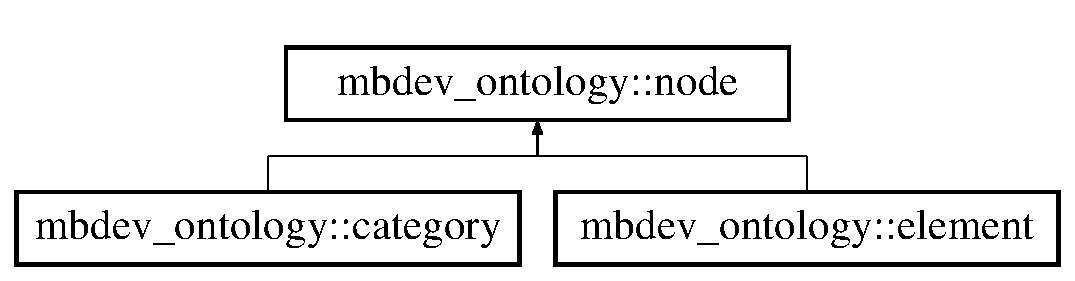
\includegraphics[height=2.000000cm]{classmbdev__ontology_1_1node}
\end{center}
\end{figure}
\subsection*{\-Public \-Member \-Functions}
\begin{DoxyCompactItemize}
\item 
\hypertarget{classmbdev__ontology_1_1node_a7d8a3f7211507f8e57bda5fd7e0e3f9d}{{\bfseries node} (\hyperlink{classmbdev_1_1string}{string} \&\hyperlink{classmbdev__ontology_1_1node_a0f69893fcec007d0766997400830a204}{name})}\label{classmbdev__ontology_1_1node_a7d8a3f7211507f8e57bda5fd7e0e3f9d}

\item 
\hypertarget{classmbdev__ontology_1_1node_af8c3f44952355f5f209836406eca80c5}{{\bfseries node} (\hyperlink{classmbdev_1_1string}{string} \&\hyperlink{classmbdev__ontology_1_1node_a0f69893fcec007d0766997400830a204}{name}, \hyperlink{classmbdev_1_1string}{string} \&\hyperlink{classmbdev__ontology_1_1node_a8af5c00f684a8c06ceeddd0a2b1ff97c}{friendly\-Name})}\label{classmbdev__ontology_1_1node_af8c3f44952355f5f209836406eca80c5}

\item 
\hypertarget{classmbdev__ontology_1_1node_af9c3b3d6c99d66a84ae5764d85da0482}{\hyperlink{classmbdev_1_1string}{string} {\bfseries get\-Name} () const }\label{classmbdev__ontology_1_1node_af9c3b3d6c99d66a84ae5764d85da0482}

\item 
\hypertarget{classmbdev__ontology_1_1node_a97e399bd609566d8be286aca9738592e}{void {\bfseries set\-Name} (\hyperlink{classmbdev_1_1string}{string} \&\hyperlink{classmbdev__ontology_1_1node_a0f69893fcec007d0766997400830a204}{name})}\label{classmbdev__ontology_1_1node_a97e399bd609566d8be286aca9738592e}

\item 
\hypertarget{classmbdev__ontology_1_1node_a00898ce49369666515ac4aefda9568e5}{\hyperlink{classmbdev_1_1string}{string} {\bfseries get\-Friendly\-Name} () const }\label{classmbdev__ontology_1_1node_a00898ce49369666515ac4aefda9568e5}

\item 
\hypertarget{classmbdev__ontology_1_1node_a0f053b86ab81be40db51fb8991f19769}{void {\bfseries set\-Friendly\-Name} (\hyperlink{classmbdev_1_1string}{string} \&freindly\-Name)}\label{classmbdev__ontology_1_1node_a0f053b86ab81be40db51fb8991f19769}

\end{DoxyCompactItemize}
\subsection*{\-Protected \-Attributes}
\begin{DoxyCompactItemize}
\item 
\hypertarget{classmbdev__ontology_1_1node_a0f69893fcec007d0766997400830a204}{\hyperlink{classmbdev_1_1string}{string} \hyperlink{classmbdev__ontology_1_1node_a0f69893fcec007d0766997400830a204}{name}}\label{classmbdev__ontology_1_1node_a0f69893fcec007d0766997400830a204}

\begin{DoxyCompactList}\small\item\em a name used to identify the object when using text mode \end{DoxyCompactList}\item 
\hypertarget{classmbdev__ontology_1_1node_a8af5c00f684a8c06ceeddd0a2b1ff97c}{\hyperlink{classmbdev_1_1string}{string} \hyperlink{classmbdev__ontology_1_1node_a8af5c00f684a8c06ceeddd0a2b1ff97c}{friendly\-Name}}\label{classmbdev__ontology_1_1node_a8af5c00f684a8c06ceeddd0a2b1ff97c}

\begin{DoxyCompactList}\small\item\em name used when the object is displayed in graphical mode \end{DoxyCompactList}\end{DoxyCompactItemize}
\subsection*{\-Friends}
\begin{DoxyCompactItemize}
\item 
\hypertarget{classmbdev__ontology_1_1node_a08a0daf86ffe80f5be310117af4235a9}{std\-::ostream \& {\bfseries operator$<$$<$} (std\-::ostream \&os, const \hyperlink{classmbdev__ontology_1_1node}{node} \&n)}\label{classmbdev__ontology_1_1node_a08a0daf86ffe80f5be310117af4235a9}

\end{DoxyCompactItemize}


\subsection{\-Detailed \-Description}
\-Contains common behaviour of \-Element and \-Relation. 

\-The documentation for this class was generated from the following files\-:\begin{DoxyCompactItemize}
\item 
/media/projects/cpp/\-Graf\-Onto/src/ontology/node.\-h\item 
/media/projects/cpp/\-Graf\-Onto/src/ontology/node.\-cpp\end{DoxyCompactItemize}

\hypertarget{classmbdev__ontology_1_1ontology}{\section{mbdev\-\_\-ontology\-:\-:ontology \-Class \-Reference}
\label{classmbdev__ontology_1_1ontology}\index{mbdev\-\_\-ontology\-::ontology@{mbdev\-\_\-ontology\-::ontology}}
}


\-A network of possibly connected concepts. \-Concepts are organized into \-Elements, and these are organized into \-Categories. \-Each \-Element belongs to exactly one \-Category. \-Elements are then joined together into groups called \-Cells. \-A \-Cell contains at most one element of every category defined in the ontology.  




{\ttfamily \#include $<$ontology.\-h$>$}

\subsection*{\-Public \-Member \-Functions}
\begin{DoxyCompactItemize}
\item 
\hypertarget{classmbdev__ontology_1_1ontology_ae12bee76ef6eb38b770afa9377fa37ad}{\hyperlink{classmbdev__ontology_1_1ontology_ae12bee76ef6eb38b770afa9377fa37ad}{ontology} ()}\label{classmbdev__ontology_1_1ontology_ae12bee76ef6eb38b770afa9377fa37ad}

\begin{DoxyCompactList}\small\item\em \-Constructs an empty ontology. \end{DoxyCompactList}\item 
\hyperlink{classmbdev_1_1string}{string} \hyperlink{classmbdev__ontology_1_1ontology_a9b2644fa7844b5024bc1c03273e0912d}{add\-Category} (\hyperlink{classmbdev_1_1string}{string} \&name)
\begin{DoxyCompactList}\small\item\em \-Constructs an ontology that has given categories. \end{DoxyCompactList}\item 
\hypertarget{classmbdev__ontology_1_1ontology_aeadc577d640dec083d2f724a05615777}{\hyperlink{classmbdev_1_1string}{string} \hyperlink{classmbdev__ontology_1_1ontology_aeadc577d640dec083d2f724a05615777}{add\-Categories} (\hyperlink{classmbdev_1_1string__vector}{string\-\_\-vector} \&names)}\label{classmbdev__ontology_1_1ontology_aeadc577d640dec083d2f724a05615777}

\begin{DoxyCompactList}\small\item\em \-Adds multiple categories at once. \end{DoxyCompactList}\item 
\hyperlink{classmbdev_1_1string}{string} \hyperlink{classmbdev__ontology_1_1ontology_aeb353a93019334cdcf01a1c9508077a7}{add\-Element} (\hyperlink{classmbdev_1_1string}{string} \&kind, \hyperlink{classmbdev_1_1string}{string} \&name)
\begin{DoxyCompactList}\small\item\em \-Adds a new element to the ontology definitions list. \end{DoxyCompactList}\item 
\hypertarget{classmbdev__ontology_1_1ontology_ab6e37f2d5c7bbdc54ca95c24c735efae}{\hyperlink{classmbdev_1_1string}{string} {\bfseries add\-Elements} (\hyperlink{classmbdev_1_1string}{string} \&kind, \hyperlink{classmbdev_1_1string__vector}{string\-\_\-vector} \&names)}\label{classmbdev__ontology_1_1ontology_ab6e37f2d5c7bbdc54ca95c24c735efae}

\item 
\hyperlink{classmbdev__ontology_1_1cell}{cell} $\ast$ \hyperlink{classmbdev__ontology_1_1ontology_a7d7f23014828019de67edb9b3a2166bb}{add\-Cell} (const \hyperlink{classmbdev__ontology_1_1cell}{cell} \&\hyperlink{classmbdev__ontology_1_1cell}{cell})
\begin{DoxyCompactList}\small\item\em \-Adds a cell to the list of defined cells. \end{DoxyCompactList}\item 
\hypertarget{classmbdev__ontology_1_1ontology_a38f19c93a3f6e817dd617fe64598c35e}{\hyperlink{classmbdev_1_1string}{string} \hyperlink{classmbdev__ontology_1_1ontology_a38f19c93a3f6e817dd617fe64598c35e}{add\-Statement} (\hyperlink{classmbdev__ontology_1_1cell}{cell} \&left, \hyperlink{classmbdev__ontology_1_1cell}{cell} \&right)}\label{classmbdev__ontology_1_1ontology_a38f19c93a3f6e817dd617fe64598c35e}

\begin{DoxyCompactList}\small\item\em \-Adds a new statement. \-If a statement exists it is first looking for. \end{DoxyCompactList}\item 
\hypertarget{classmbdev__ontology_1_1ontology_ac8c5ca3059987b8bb4bb7e35bb7d27bc}{\hyperlink{classmbdev_1_1string}{string} {\bfseries delete\-Category} (const \hyperlink{classmbdev_1_1string}{string} \&name)}\label{classmbdev__ontology_1_1ontology_ac8c5ca3059987b8bb4bb7e35bb7d27bc}

\item 
\hypertarget{classmbdev__ontology_1_1ontology_ac923a46fd1212a4778f6ab77468376e3}{\hyperlink{classmbdev_1_1string}{string} {\bfseries delete\-Element} (const \hyperlink{classmbdev_1_1string}{string} \&name)}\label{classmbdev__ontology_1_1ontology_ac923a46fd1212a4778f6ab77468376e3}

\item 
\hypertarget{classmbdev__ontology_1_1ontology_a27de6b3b8c0507c9b5383b16cfc23552}{\hyperlink{classmbdev__ontology_1_1category}{category} $\ast$ \hyperlink{classmbdev__ontology_1_1ontology_a27de6b3b8c0507c9b5383b16cfc23552}{find\-Category} (const \hyperlink{classmbdev_1_1string}{string} \&name)}\label{classmbdev__ontology_1_1ontology_a27de6b3b8c0507c9b5383b16cfc23552}

\begin{DoxyCompactList}\small\item\em \-Looks for a category that has the given name and returns its address. \end{DoxyCompactList}\item 
\hypertarget{classmbdev__ontology_1_1ontology_aa77f2ba5499396a15c598e39ce86912c}{int {\bfseries get\-Category\-Index} (const \hyperlink{classmbdev_1_1string}{string} \&name)}\label{classmbdev__ontology_1_1ontology_aa77f2ba5499396a15c598e39ce86912c}

\item 
\hypertarget{classmbdev__ontology_1_1ontology_a9dae61dce79833a83c7361b72f435c44}{\hyperlink{classmbdev__ontology_1_1element}{element} $\ast$ \hyperlink{classmbdev__ontology_1_1ontology_a9dae61dce79833a83c7361b72f435c44}{find\-Element} (const \hyperlink{classmbdev_1_1string}{string} \&name)}\label{classmbdev__ontology_1_1ontology_a9dae61dce79833a83c7361b72f435c44}

\begin{DoxyCompactList}\small\item\em \-Looks for an element that has the given name and returns its address. \end{DoxyCompactList}\item 
\hypertarget{classmbdev__ontology_1_1ontology_a612e5dd67fcac3a09b1a706afd109302}{\hyperlink{classmbdev_1_1ptr__vector}{ptr\-\_\-vector}$<$ \hyperlink{classmbdev__ontology_1_1element}{element} $>$ {\bfseries find\-Elements} (const \hyperlink{classmbdev_1_1string}{string} \&kind)}\label{classmbdev__ontology_1_1ontology_a612e5dd67fcac3a09b1a706afd109302}

\item 
\hypertarget{classmbdev__ontology_1_1ontology_a9954a0577b6954559a30de87ca9e87cd}{int {\bfseries get\-Element\-Index} (const \hyperlink{classmbdev_1_1string}{string} \&name) const }\label{classmbdev__ontology_1_1ontology_a9954a0577b6954559a30de87ca9e87cd}

\item 
\hypertarget{classmbdev__ontology_1_1ontology_ae9844b5e7d13a76b8047da14d1111589}{\hyperlink{classmbdev_1_1ptr__vector}{ptr\-\_\-vector}$<$ int $>$ {\bfseries get\-Element\-Indexes} (const \hyperlink{classmbdev_1_1string}{string} \&kind) const }\label{classmbdev__ontology_1_1ontology_ae9844b5e7d13a76b8047da14d1111589}

\item 
\hypertarget{classmbdev__ontology_1_1ontology_a84485b7f8554e5998481f391c82fb758}{\hyperlink{classmbdev_1_1ptr__vector}{ptr\-\_\-vector}$<$ \hyperlink{classmbdev__ontology_1_1cell}{cell} $>$ \hyperlink{classmbdev__ontology_1_1ontology_a84485b7f8554e5998481f391c82fb758}{find\-Cells} (const \hyperlink{classmbdev__ontology_1_1cell}{cell} \&matching, bool exact=false)}\label{classmbdev__ontology_1_1ontology_a84485b7f8554e5998481f391c82fb758}

\begin{DoxyCompactList}\small\item\em \-Looks for cells that are matching the given one and returns their address. \end{DoxyCompactList}\item 
\hypertarget{classmbdev__ontology_1_1ontology_a5b9977beda0a587e56e34d9a94d8c937}{\hyperlink{classmbdev_1_1ptr__vector}{ptr\-\_\-vector}$<$ \hyperlink{classmbdev__ontology_1_1cell}{cell} $>$ {\bfseries find\-Cells} ()}\label{classmbdev__ontology_1_1ontology_a5b9977beda0a587e56e34d9a94d8c937}

\item 
\hypertarget{classmbdev__ontology_1_1ontology_acc8d92197dc8b96180c1f1e33cff6a67}{\hyperlink{classmbdev_1_1ptr__vector}{ptr\-\_\-vector}$<$ \hyperlink{classmbdev__ontology_1_1statement}{statement} $>$ \hyperlink{classmbdev__ontology_1_1ontology_acc8d92197dc8b96180c1f1e33cff6a67}{find\-Statements} (\hyperlink{classmbdev__ontology_1_1statement}{statement} \&matching, bool ignore\-Transitivity=false)}\label{classmbdev__ontology_1_1ontology_acc8d92197dc8b96180c1f1e33cff6a67}

\begin{DoxyCompactList}\small\item\em \-Looks for a category that has the given name and returns its address. \end{DoxyCompactList}\item 
\hypertarget{classmbdev__ontology_1_1ontology_adefeb11a57e891c9f0195dc3e57e46a0}{\hyperlink{classmbdev_1_1string__vector}{string\-\_\-vector} {\bfseries get\-Categories} () const }\label{classmbdev__ontology_1_1ontology_adefeb11a57e891c9f0195dc3e57e46a0}

\item 
\hypertarget{classmbdev__ontology_1_1ontology_a978a41f8f81f6fd330ae678b22d66ef4}{\hyperlink{classmbdev_1_1string__vector}{string\-\_\-vector} {\bfseries get\-Elements} () const }\label{classmbdev__ontology_1_1ontology_a978a41f8f81f6fd330ae678b22d66ef4}

\item 
\hypertarget{classmbdev__ontology_1_1ontology_a68fd8a8730f58589c8e39e6611d247e7}{\hyperlink{classmbdev_1_1string__vector}{string\-\_\-vector} {\bfseries get\-Cells} () const }\label{classmbdev__ontology_1_1ontology_a68fd8a8730f58589c8e39e6611d247e7}

\item 
\hypertarget{classmbdev__ontology_1_1ontology_ac7ac79e55a7b0914cad5f14156ab2cda}{\hyperlink{classmbdev_1_1string}{string} {\bfseries to\-String} () const }\label{classmbdev__ontology_1_1ontology_ac7ac79e55a7b0914cad5f14156ab2cda}

\end{DoxyCompactItemize}
\subsection*{\-Protected \-Attributes}
\begin{DoxyCompactItemize}
\item 
\hypertarget{classmbdev__ontology_1_1ontology_afe40885a5e07d5c03a85d1112be0af4b}{\hyperlink{classmbdev_1_1ptr__vector}{ptr\-\_\-vector}$<$ \hyperlink{classmbdev__ontology_1_1statement}{statement} $>$ \hyperlink{classmbdev__ontology_1_1ontology_afe40885a5e07d5c03a85d1112be0af4b}{statements}}\label{classmbdev__ontology_1_1ontology_afe40885a5e07d5c03a85d1112be0af4b}

\begin{DoxyCompactList}\small\item\em \-List of statements that makes up the ontology. \end{DoxyCompactList}\end{DoxyCompactItemize}
\subsection*{\-Friends}
\begin{DoxyCompactItemize}
\item 
\hypertarget{classmbdev__ontology_1_1ontology_a75cf9be86fe5d94bad68d0dd50684ce6}{std\-::ostream \& {\bfseries operator$<$$<$} (std\-::ostream \&os, const \hyperlink{classmbdev__ontology_1_1ontology}{ontology} \&o)}\label{classmbdev__ontology_1_1ontology_a75cf9be86fe5d94bad68d0dd50684ce6}

\end{DoxyCompactItemize}


\subsection{\-Detailed \-Description}
\-A network of possibly connected concepts. \-Concepts are organized into \-Elements, and these are organized into \-Categories. \-Each \-Element belongs to exactly one \-Category. \-Elements are then joined together into groups called \-Cells. \-A \-Cell contains at most one element of every category defined in the ontology. 

\subsection{\-Member \-Function \-Documentation}
\hypertarget{classmbdev__ontology_1_1ontology_a9b2644fa7844b5024bc1c03273e0912d}{\index{mbdev\-\_\-ontology\-::ontology@{mbdev\-\_\-ontology\-::ontology}!add\-Category@{add\-Category}}
\index{add\-Category@{add\-Category}!mbdev_ontology::ontology@{mbdev\-\_\-ontology\-::ontology}}
\subsubsection[{add\-Category}]{\setlength{\rightskip}{0pt plus 5cm}{\bf string} {\bf mbdev\-\_\-ontology\-::ontology\-::add\-Category} (
\begin{DoxyParamCaption}
\item[{{\bf string} \&}]{name}
\end{DoxyParamCaption}
)}}\label{classmbdev__ontology_1_1ontology_a9b2644fa7844b5024bc1c03273e0912d}


\-Constructs an ontology that has given categories. 


\begin{DoxyParams}{\-Parameters}
{\em categories} & array of names of the categories\\
\hline
\end{DoxyParams}
\-Adds a new property to the ontology definitions list. 
\begin{DoxyParams}{\-Parameters}
{\em name} & name of the new property \\
\hline
\end{DoxyParams}
\hypertarget{classmbdev__ontology_1_1ontology_a7d7f23014828019de67edb9b3a2166bb}{\index{mbdev\-\_\-ontology\-::ontology@{mbdev\-\_\-ontology\-::ontology}!add\-Cell@{add\-Cell}}
\index{add\-Cell@{add\-Cell}!mbdev_ontology::ontology@{mbdev\-\_\-ontology\-::ontology}}
\subsubsection[{add\-Cell}]{\setlength{\rightskip}{0pt plus 5cm}{\bf cell} $\ast$ {\bf mbdev\-\_\-ontology\-::ontology\-::add\-Cell} (
\begin{DoxyParamCaption}
\item[{const {\bf cell} \&}]{cell}
\end{DoxyParamCaption}
)}}\label{classmbdev__ontology_1_1ontology_a7d7f23014828019de67edb9b3a2166bb}


\-Adds a cell to the list of defined cells. 


\begin{DoxyParams}{\-Parameters}
{\em cell} & \\
\hline
\end{DoxyParams}
\begin{DoxyReturn}{\-Returns}
address of a cell that was actually stored in the ontology 
\end{DoxyReturn}
\hypertarget{classmbdev__ontology_1_1ontology_aeb353a93019334cdcf01a1c9508077a7}{\index{mbdev\-\_\-ontology\-::ontology@{mbdev\-\_\-ontology\-::ontology}!add\-Element@{add\-Element}}
\index{add\-Element@{add\-Element}!mbdev_ontology::ontology@{mbdev\-\_\-ontology\-::ontology}}
\subsubsection[{add\-Element}]{\setlength{\rightskip}{0pt plus 5cm}{\bf string} {\bf mbdev\-\_\-ontology\-::ontology\-::add\-Element} (
\begin{DoxyParamCaption}
\item[{{\bf string} \&}]{kind, }
\item[{{\bf string} \&}]{name}
\end{DoxyParamCaption}
)}}\label{classmbdev__ontology_1_1ontology_aeb353a93019334cdcf01a1c9508077a7}


\-Adds a new element to the ontology definitions list. 


\begin{DoxyParams}{\-Parameters}
{\em kind} & property, to which given value will be assigned \\
\hline
{\em name} & name of the new element \\
\hline
\end{DoxyParams}


\-The documentation for this class was generated from the following files\-:\begin{DoxyCompactItemize}
\item 
/media/projects/cpp/\-Graf\-Onto/src/ontology/ontology.\-h\item 
/media/projects/cpp/\-Graf\-Onto/src/ontology/ontology.\-cpp\end{DoxyCompactItemize}

\hypertarget{classmbdev_1_1ptr__vector}{\section{mbdev\-:\-:ptr\-\_\-vector$<$ \-T $>$ \-Class \-Template \-Reference}
\label{classmbdev_1_1ptr__vector}\index{mbdev\-::ptr\-\_\-vector$<$ T $>$@{mbdev\-::ptr\-\_\-vector$<$ T $>$}}
}
\-Inheritance diagram for mbdev\-:\-:ptr\-\_\-vector$<$ \-T $>$\-:\begin{figure}[H]
\begin{center}
\leavevmode
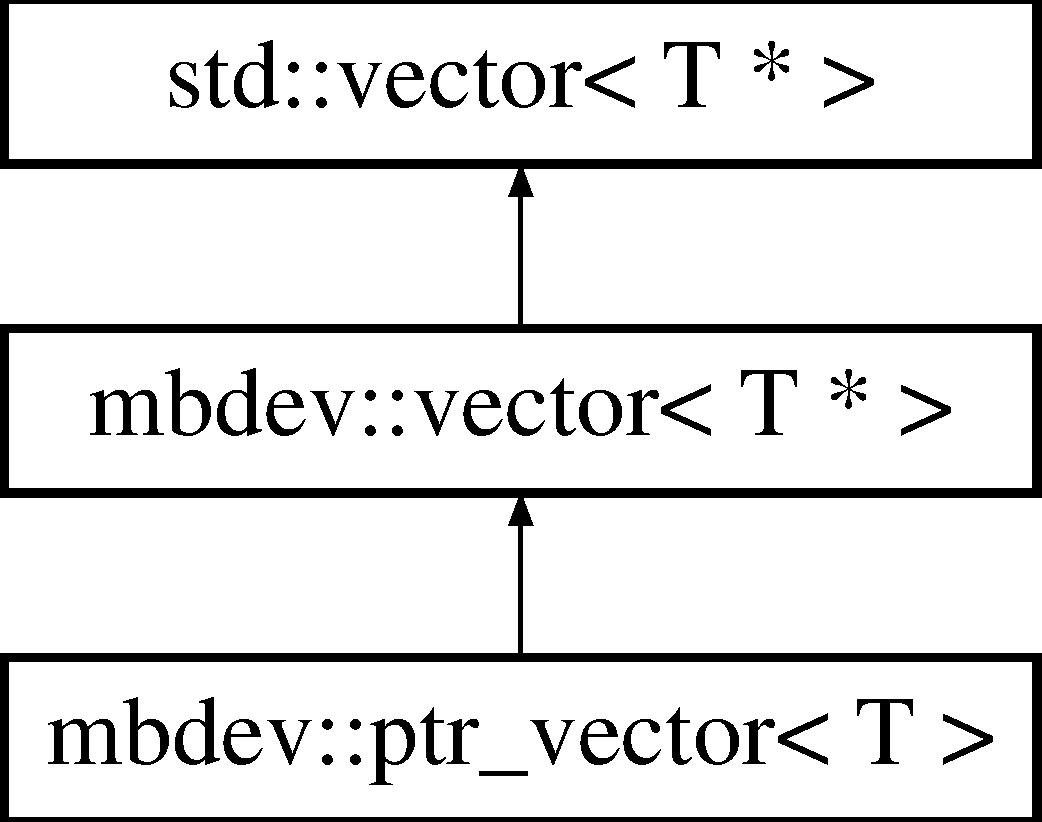
\includegraphics[height=3.000000cm]{classmbdev_1_1ptr__vector}
\end{center}
\end{figure}
\subsection*{\-Public \-Member \-Functions}
\begin{DoxyCompactItemize}
\item 
\hypertarget{classmbdev_1_1ptr__vector_ab35e93145913085d1c05afab6be17a1e}{virtual std\-::string {\bfseries to\-String} ()}\label{classmbdev_1_1ptr__vector_ab35e93145913085d1c05afab6be17a1e}

\end{DoxyCompactItemize}
\subsubsection*{template$<$typename \-T$>$ class mbdev\-::ptr\-\_\-vector$<$ T $>$}



\-The documentation for this class was generated from the following file\-:\begin{DoxyCompactItemize}
\item 
/media/projects/cpp/\-Graf\-Onto/src/mbdev/ptr\-\_\-vector.\-h\end{DoxyCompactItemize}

\hypertarget{classmbdev__ontology_1_1statement}{\section{mbdev\-\_\-ontology\-:\-:statement \-Class \-Reference}
\label{classmbdev__ontology_1_1statement}\index{mbdev\-\_\-ontology\-::statement@{mbdev\-\_\-ontology\-::statement}}
}


\-Used to store a single statement of an ontology. \-Statement is a pair of cells.  




{\ttfamily \#include $<$statement.\-h$>$}

\subsection*{\-Public \-Member \-Functions}
\begin{DoxyCompactItemize}
\item 
\hypertarget{classmbdev__ontology_1_1statement_a29debd9185df2ae9c4a26e2631d64060}{{\bfseries statement} (\hyperlink{classmbdev__ontology_1_1cell}{cell} $\ast$left\-Side, \hyperlink{classmbdev__ontology_1_1cell}{cell} $\ast$right\-Side)}\label{classmbdev__ontology_1_1statement_a29debd9185df2ae9c4a26e2631d64060}

\item 
\hypertarget{classmbdev__ontology_1_1statement_a5d20463fc12a458be62b0d70ee5259fd}{\hyperlink{classmbdev__ontology_1_1cell}{cell} \& {\bfseries left} ()}\label{classmbdev__ontology_1_1statement_a5d20463fc12a458be62b0d70ee5259fd}

\item 
\hypertarget{classmbdev__ontology_1_1statement_ae06d865de61bb924b8b1827d1b301ae4}{\hyperlink{classmbdev__ontology_1_1cell}{cell} \& {\bfseries right} ()}\label{classmbdev__ontology_1_1statement_ae06d865de61bb924b8b1827d1b301ae4}

\item 
\hypertarget{classmbdev__ontology_1_1statement_ac4ab8b4d7fa0c6b42c33f04490c33e76}{\hyperlink{classmbdev__ontology_1_1cell}{cell} $\ast$ {\bfseries left\-Ptr} ()}\label{classmbdev__ontology_1_1statement_ac4ab8b4d7fa0c6b42c33f04490c33e76}

\item 
\hypertarget{classmbdev__ontology_1_1statement_af1a1d7dd1c299aea445765a3fd65dc14}{\hyperlink{classmbdev__ontology_1_1cell}{cell} $\ast$ {\bfseries right\-Ptr} ()}\label{classmbdev__ontology_1_1statement_af1a1d7dd1c299aea445765a3fd65dc14}

\end{DoxyCompactItemize}
\subsection*{\-Friends}
\begin{DoxyCompactItemize}
\item 
\hypertarget{classmbdev__ontology_1_1statement_a7aabf5e95163ab47ab639660ec084aad}{std\-::ostream \& {\bfseries operator$<$$<$} (std\-::ostream \&os, const \hyperlink{classmbdev__ontology_1_1statement}{statement} \&s)}\label{classmbdev__ontology_1_1statement_a7aabf5e95163ab47ab639660ec084aad}

\end{DoxyCompactItemize}


\subsection{\-Detailed \-Description}
\-Used to store a single statement of an ontology. \-Statement is a pair of cells. 

\-The documentation for this class was generated from the following files\-:\begin{DoxyCompactItemize}
\item 
/media/projects/cpp/\-Graf\-Onto/src/ontology/statement.\-h\item 
/media/projects/cpp/\-Graf\-Onto/src/ontology/statement.\-cpp\end{DoxyCompactItemize}

\hypertarget{classmbdev_1_1string}{\section{mbdev\-:\-:string \-Class \-Reference}
\label{classmbdev_1_1string}\index{mbdev\-::string@{mbdev\-::string}}
}
\subsection*{\-Public \-Member \-Functions}
\begin{DoxyCompactItemize}
\item 
\hypertarget{classmbdev_1_1string_a346dc571197f1e56d6bf0cfc1b717683}{{\bfseries string} (const char source)}\label{classmbdev_1_1string_a346dc571197f1e56d6bf0cfc1b717683}

\item 
\hypertarget{classmbdev_1_1string_a42a1cf2ce3836cc4f30f71a905173127}{{\bfseries string} (const char $\ast$source)}\label{classmbdev_1_1string_a42a1cf2ce3836cc4f30f71a905173127}

\item 
\hypertarget{classmbdev_1_1string_a9e8ea6a1421176521dae10ca21f157d9}{{\bfseries string} (const std\-::string \&source)}\label{classmbdev_1_1string_a9e8ea6a1421176521dae10ca21f157d9}

\item 
\hypertarget{classmbdev_1_1string_a41cc2cfdacaa7d2db1e85cc1b5119422}{{\bfseries string} (const \hyperlink{classmbdev_1_1string}{string} \&source)}\label{classmbdev_1_1string_a41cc2cfdacaa7d2db1e85cc1b5119422}

\item 
\hyperlink{classmbdev_1_1string}{string} \& \hyperlink{classmbdev_1_1string_ab673feed85f4b0a582ba7c0797ef99a9}{ltrim} ()
\begin{DoxyCompactList}\small\item\em \-Trims a given string from start. \end{DoxyCompactList}\item 
\hyperlink{classmbdev_1_1string}{string} \& \hyperlink{classmbdev_1_1string_acd0647d477fc2fd71cf4902423075000}{rtrim} ()
\begin{DoxyCompactList}\small\item\em \-Trims a given string from end. \end{DoxyCompactList}\item 
\hyperlink{classmbdev_1_1string}{string} \& \hyperlink{classmbdev_1_1string_a5f8b27d5a309c9c5acb58e741b046438}{trim} ()
\begin{DoxyCompactList}\small\item\em \-Trims a given string from both ends. \end{DoxyCompactList}\item 
\hypertarget{classmbdev_1_1string_a16d301549852cd8beb980f04ae4575f4}{bool {\bfseries equals} (const \hyperlink{classmbdev_1_1string}{string} \&s) const }\label{classmbdev_1_1string_a16d301549852cd8beb980f04ae4575f4}

\item 
\hyperlink{classmbdev_1_1string__vector}{string\-\_\-vector} \hyperlink{classmbdev_1_1string_a32e61d95ec60bc8c9a419551284278aa}{to\-Vector} (const char separator) const 
\begin{DoxyCompactList}\small\item\em \-Makes a string vector out of string with separators and a sample of a separator. \-If a symbol is a separator it can't be at the same time used as a symbol in any member substring. \end{DoxyCompactList}\end{DoxyCompactItemize}
\subsection*{\-Static \-Public \-Attributes}
\begin{DoxyCompactItemize}
\item 
\hypertarget{classmbdev_1_1string_abe8e7c5dd8a04459bb1f323c9fd54f2a}{static const std\-::string \hyperlink{classmbdev_1_1string_abe8e7c5dd8a04459bb1f323c9fd54f2a}{empty\-Std\-Str} = std\-::string()}\label{classmbdev_1_1string_abe8e7c5dd8a04459bb1f323c9fd54f2a}

\begin{DoxyCompactList}\small\item\em \-Std string of length zero. \end{DoxyCompactList}\item 
\hypertarget{classmbdev_1_1string_af3502d5e7550b0328ce963f6e32d6856}{static const \hyperlink{classmbdev_1_1string}{string} \hyperlink{classmbdev_1_1string_af3502d5e7550b0328ce963f6e32d6856}{empty\-Str} = \hyperlink{classmbdev_1_1string}{string}()}\label{classmbdev_1_1string_af3502d5e7550b0328ce963f6e32d6856}

\begin{DoxyCompactList}\small\item\em \-String of length zero. \end{DoxyCompactList}\end{DoxyCompactItemize}
\subsection*{\-Friends}
\begin{DoxyCompactItemize}
\item 
\hypertarget{classmbdev_1_1string_ab3a419ebbe25751e69a82233c9d11310}{std\-::ostream \& {\bfseries operator$<$$<$} (std\-::ostream \&os, const \hyperlink{classmbdev_1_1string}{string} \&s)}\label{classmbdev_1_1string_ab3a419ebbe25751e69a82233c9d11310}

\end{DoxyCompactItemize}


\subsection{\-Member \-Function \-Documentation}
\hypertarget{classmbdev_1_1string_ab673feed85f4b0a582ba7c0797ef99a9}{\index{mbdev\-::string@{mbdev\-::string}!ltrim@{ltrim}}
\index{ltrim@{ltrim}!mbdev::string@{mbdev\-::string}}
\subsubsection[{ltrim}]{\setlength{\rightskip}{0pt plus 5cm}{\bf string} \& {\bf mbdev\-::string\-::ltrim} (
\begin{DoxyParamCaption}
{}
\end{DoxyParamCaption}
)\hspace{0.3cm}{\ttfamily  \mbox{[}inline\mbox{]}}}}\label{classmbdev_1_1string_ab673feed85f4b0a582ba7c0797ef99a9}


\-Trims a given string from start. 

\begin{DoxyReturn}{\-Returns}
reference to the same string 
\end{DoxyReturn}
\hypertarget{classmbdev_1_1string_acd0647d477fc2fd71cf4902423075000}{\index{mbdev\-::string@{mbdev\-::string}!rtrim@{rtrim}}
\index{rtrim@{rtrim}!mbdev::string@{mbdev\-::string}}
\subsubsection[{rtrim}]{\setlength{\rightskip}{0pt plus 5cm}{\bf string} \& {\bf mbdev\-::string\-::rtrim} (
\begin{DoxyParamCaption}
{}
\end{DoxyParamCaption}
)\hspace{0.3cm}{\ttfamily  \mbox{[}inline\mbox{]}}}}\label{classmbdev_1_1string_acd0647d477fc2fd71cf4902423075000}


\-Trims a given string from end. 

\begin{DoxyReturn}{\-Returns}
reference to the same string 
\end{DoxyReturn}
\hypertarget{classmbdev_1_1string_a32e61d95ec60bc8c9a419551284278aa}{\index{mbdev\-::string@{mbdev\-::string}!to\-Vector@{to\-Vector}}
\index{to\-Vector@{to\-Vector}!mbdev::string@{mbdev\-::string}}
\subsubsection[{to\-Vector}]{\setlength{\rightskip}{0pt plus 5cm}{\bf string\-\_\-vector} {\bf mbdev\-::string\-::to\-Vector} (
\begin{DoxyParamCaption}
\item[{const char}]{separator}
\end{DoxyParamCaption}
) const}}\label{classmbdev_1_1string_a32e61d95ec60bc8c9a419551284278aa}


\-Makes a string vector out of string with separators and a sample of a separator. \-If a symbol is a separator it can't be at the same time used as a symbol in any member substring. 


\begin{DoxyParams}{\-Parameters}
{\em separator} & the separator \\
\hline
\end{DoxyParams}
\hypertarget{classmbdev_1_1string_a5f8b27d5a309c9c5acb58e741b046438}{\index{mbdev\-::string@{mbdev\-::string}!trim@{trim}}
\index{trim@{trim}!mbdev::string@{mbdev\-::string}}
\subsubsection[{trim}]{\setlength{\rightskip}{0pt plus 5cm}{\bf string} \& {\bf mbdev\-::string\-::trim} (
\begin{DoxyParamCaption}
{}
\end{DoxyParamCaption}
)\hspace{0.3cm}{\ttfamily  \mbox{[}inline\mbox{]}}}}\label{classmbdev_1_1string_a5f8b27d5a309c9c5acb58e741b046438}


\-Trims a given string from both ends. 

\begin{DoxyReturn}{\-Returns}
reference to the same string 
\end{DoxyReturn}


\-The documentation for this class was generated from the following files\-:\begin{DoxyCompactItemize}
\item 
/media/projects/cpp/\-Graf\-Onto/src/mbdev/string.\-h\item 
/media/projects/cpp/\-Graf\-Onto/src/mbdev/string.\-cpp\end{DoxyCompactItemize}

\hypertarget{classmbdev_1_1string__vector}{\section{mbdev\-:\-:string\-\_\-vector \-Class \-Reference}
\label{classmbdev_1_1string__vector}\index{mbdev\-::string\-\_\-vector@{mbdev\-::string\-\_\-vector}}
}
\-Inheritance diagram for mbdev\-:\-:string\-\_\-vector\-:\begin{figure}[H]
\begin{center}
\leavevmode
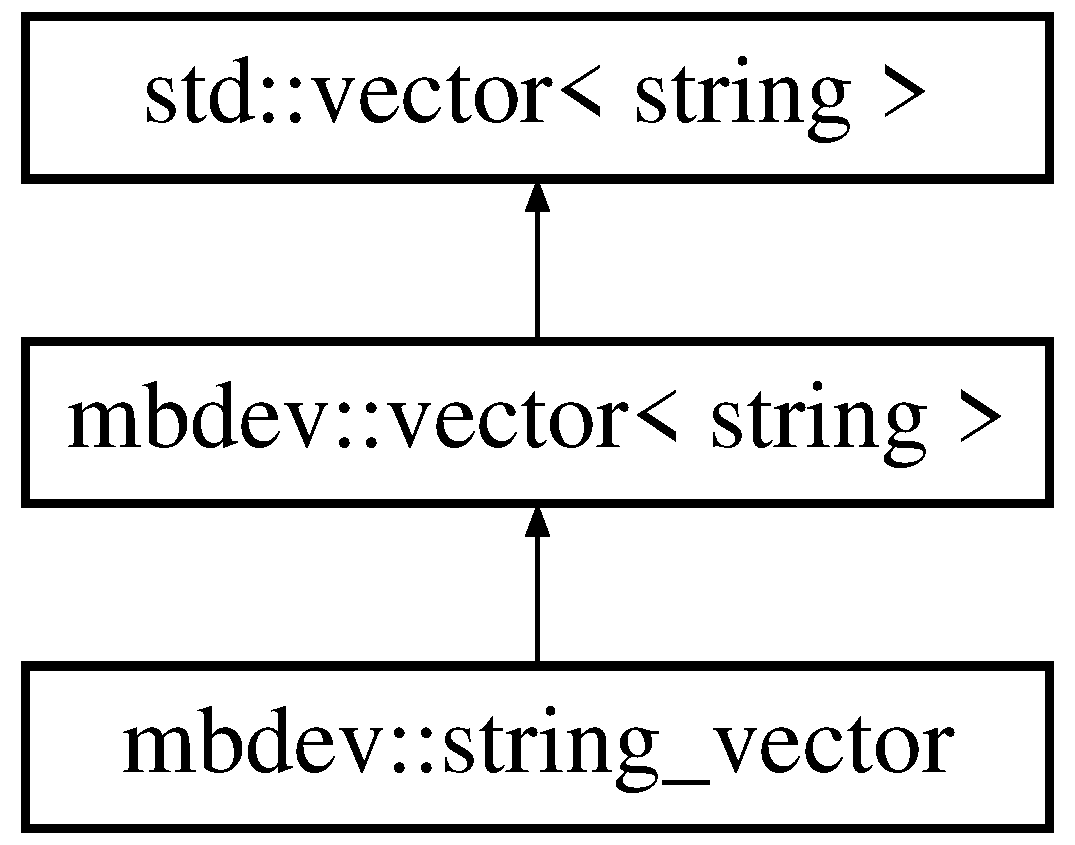
\includegraphics[height=3.000000cm]{classmbdev_1_1string__vector}
\end{center}
\end{figure}
\subsection*{\-Public \-Member \-Functions}
\begin{DoxyCompactItemize}
\item 
\hypertarget{classmbdev_1_1string__vector_a95085457cf0a524f0cf7fa4017781372}{int {\bfseries index\-Contains} (const \hyperlink{classmbdev_1_1string}{string} \&str)}\label{classmbdev_1_1string__vector_a95085457cf0a524f0cf7fa4017781372}

\item 
\hypertarget{classmbdev_1_1string__vector_a899d556cda887346b0c4ad7ad424f980}{void {\bfseries push\-\_\-back} (const \hyperlink{classmbdev_1_1string}{string} \&str)}\label{classmbdev_1_1string__vector_a899d556cda887346b0c4ad7ad424f980}

\item 
\hypertarget{classmbdev_1_1string__vector_a4e9f55d5457e441978f0d43838791947}{void {\bfseries push\-\_\-back} (int argc, const char $\ast$$\ast$argv)}\label{classmbdev_1_1string__vector_a4e9f55d5457e441978f0d43838791947}

\item 
\hypertarget{classmbdev_1_1string__vector_a79e5788b6cbbacf7ce2197557c69576e}{\hyperlink{classmbdev_1_1string__vector}{string\-\_\-vector} \& {\bfseries trim} ()}\label{classmbdev_1_1string__vector_a79e5788b6cbbacf7ce2197557c69576e}

\item 
\hypertarget{classmbdev_1_1string__vector_a2631a3889a8ff8b6fd9b9e5c761e0d9a}{\hyperlink{classmbdev_1_1string__vector}{string\-\_\-vector} \& {\bfseries cleanse} ()}\label{classmbdev_1_1string__vector_a2631a3889a8ff8b6fd9b9e5c761e0d9a}

\item 
\hypertarget{classmbdev_1_1string__vector_a9c79f3c3cbec193a841fcf79d54745d7}{\hyperlink{classmbdev_1_1string}{string} {\bfseries str} (const \hyperlink{classmbdev_1_1string}{string} \&separator, int pos=0, size\-\_\-t n=std\-::string\-::npos) const }\label{classmbdev_1_1string__vector_a9c79f3c3cbec193a841fcf79d54745d7}

\item 
\hypertarget{classmbdev_1_1string__vector_a9dae9a795bda0f5dd7154740c353ed79}{\hyperlink{classmbdev_1_1string}{string} {\bfseries str} (const char separator, int pos=0, size\-\_\-t n=std\-::string\-::npos) const }\label{classmbdev_1_1string__vector_a9dae9a795bda0f5dd7154740c353ed79}

\item 
\hypertarget{classmbdev_1_1string__vector_a7c8e1568055ee349454b477e37573a16}{\hyperlink{classmbdev_1_1string}{string} {\bfseries str} (int pos=0, size\-\_\-t n=std\-::string\-::npos) const }\label{classmbdev_1_1string__vector_a7c8e1568055ee349454b477e37573a16}

\end{DoxyCompactItemize}
\subsection*{\-Static \-Public \-Attributes}
\begin{DoxyCompactItemize}
\item 
\hypertarget{classmbdev_1_1string__vector_a217dba7ae43824ecc9da76db562fed16}{static const \hyperlink{classmbdev_1_1string__vector}{string\-\_\-vector} \hyperlink{classmbdev_1_1string__vector_a217dba7ae43824ecc9da76db562fed16}{empty} = \hyperlink{classmbdev_1_1string__vector}{string\-\_\-vector}()}\label{classmbdev_1_1string__vector_a217dba7ae43824ecc9da76db562fed16}

\begin{DoxyCompactList}\small\item\em \-S\-T\-L vector with no elements. \end{DoxyCompactList}\end{DoxyCompactItemize}


\-The documentation for this class was generated from the following files\-:\begin{DoxyCompactItemize}
\item 
/media/projects/cpp/\-Graf\-Onto/src/mbdev/string\-\_\-vector.\-h\item 
/media/projects/cpp/\-Graf\-Onto/src/mbdev/string\-\_\-vector.\-cpp\end{DoxyCompactItemize}

\hypertarget{classstd_1_1vector}{\section{vector \-Class \-Reference}
\label{classstd_1_1vector}\index{vector@{vector}}
}
\-Inheritance diagram for vector\-:\begin{figure}[H]
\begin{center}
\leavevmode
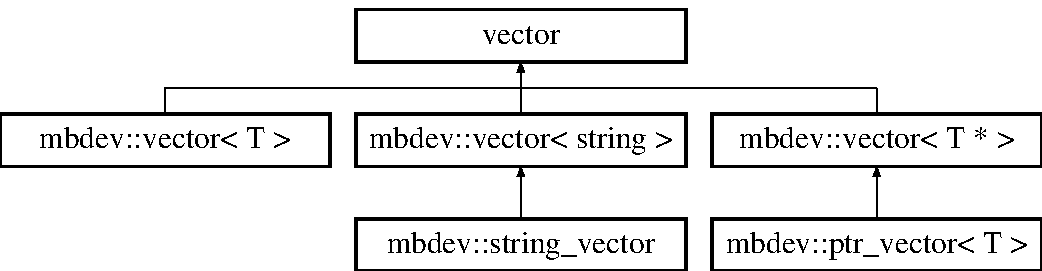
\includegraphics[height=3.000000cm]{classstd_1_1vector}
\end{center}
\end{figure}


\-The documentation for this class was generated from the following file\-:\begin{DoxyCompactItemize}
\item 
/media/projects/cpp/\-Graf\-Onto/src/mbdev/vector.\-h\end{DoxyCompactItemize}

\hypertarget{classmbdev_1_1vector}{\section{mbdev\-:\-:vector$<$ \-T $>$ \-Class \-Template \-Reference}
\label{classmbdev_1_1vector}\index{mbdev\-::vector$<$ T $>$@{mbdev\-::vector$<$ T $>$}}
}
\-Inheritance diagram for mbdev\-:\-:vector$<$ \-T $>$\-:\begin{figure}[H]
\begin{center}
\leavevmode
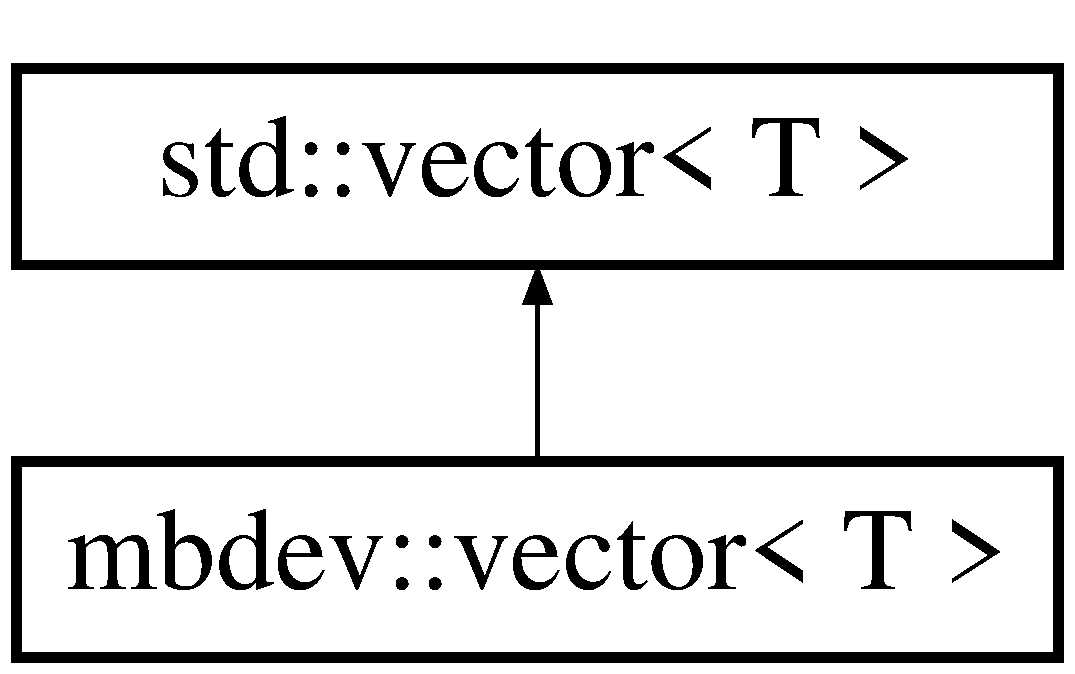
\includegraphics[height=2.000000cm]{classmbdev_1_1vector}
\end{center}
\end{figure}
\subsection*{\-Public \-Member \-Functions}
\begin{DoxyCompactItemize}
\item 
\hypertarget{classmbdev_1_1vector_a9a37ea62d9ba3d2b4a2e4928c1af82f5}{{\bfseries vector} (size\-\_\-t n)}\label{classmbdev_1_1vector_a9a37ea62d9ba3d2b4a2e4928c1af82f5}

\item 
\hypertarget{classmbdev_1_1vector_a99c3219ba4f717d34cd459636592b28b}{int {\bfseries index\-Of} (\-T element) const }\label{classmbdev_1_1vector_a99c3219ba4f717d34cd459636592b28b}

\item 
\hypertarget{classmbdev_1_1vector_a23075da46c91e0e298a5d00ad75e1a37}{virtual std\-::string {\bfseries to\-String} ()}\label{classmbdev_1_1vector_a23075da46c91e0e298a5d00ad75e1a37}

\item 
\hypertarget{classmbdev_1_1vector_a9cd033551bcfa97f72a2964e7120fdfc}{\hyperlink{classmbdev_1_1vector}{vector}$<$ \-T $>$ \& {\bfseries operator+=} (const \hyperlink{classmbdev_1_1vector}{vector}$<$ \-T $>$ \&vec)}\label{classmbdev_1_1vector_a9cd033551bcfa97f72a2964e7120fdfc}

\end{DoxyCompactItemize}
\subsubsection*{template$<$typename \-T$>$ class mbdev\-::vector$<$ T $>$}



\-The documentation for this class was generated from the following file\-:\begin{DoxyCompactItemize}
\item 
/media/projects/cpp/\-Graf\-Onto/src/mbdev/vector.\-h\end{DoxyCompactItemize}

\printindex
\end{document}
